\chapterauthor{Accumulator Design}{Paul Vogelberg}

\section{Introduction}
This report presents the accumulator design for a Formula Student electric vehicle under an acceleration-event-only scenario.

%TODO: rewrite when fitted within the rest of the group report

\subsection{Project Scope}
The design encompasses the following scope:
\begin{itemize}
    \item Technology and cell selection for an acceleration-only duty cycle.
    \item Electrical architecture at pack and segment level.
    \item FS-required in-casing electrical safety measures.
    \item AMS slave-to-master monitoring architecture and master interface to the vehicle ECU.
    \item Mechanical packaging of segment modules and accumulator container layout.
    \item Analytical verification against requirements and comparison with alternatives.
\end{itemize}

The following items are treated as out of scope for detailed derivation in this document and are stated as future or external work: all safety and charging systems outside the accumulator casing, full AMS firmware implementation, full manufacturing process planning, exhaustive scrutineering documentation, and complete physical test campaign data.

\section{Technology Selection}

\subsection{Design Requirements and Selection Criteria}
Due to the nature of the acceleration-only event, the primary design driver is peak power delivery rather than total energy capacity. This shifts the focus towards technologies with high power density.

To compare energy storage technologies, the following criteria were defined: (1) power output, (2) total energy capacity, and (3) a combined optimisation objective covering mass, volume, cost, and procurement risk.
FS Rules limit accumulator output power to 80 kW (FS-EV 7.2.4). Power can be treated as constant during the event as a conservative estimate assuming traction-limited periods are brief relative to total run time. Event duration is set to 4 s based on top Formula Student performances lasting 3.5 s.

The required energy capacity is simply calculated using:
\begin{equation*}
E = P \cdot t = 80~\text{kW} \times 4~\text{s} = 320~\text{kJ} = 89~\text{Wh}
\end{equation*}

The resulting design requirements used for downstream verification are defined in Table~\ref{tab:design_requirement_ids}.

\begin{table}[htbp]
    \centering
    \caption{Requirement table with targets for the accumulator design.}
    \label{tab:design_requirement_ids}
    \footnotesize
    \begin{tabular}{|c|l|l|}
        \hline
        \textbf{ID} & \textbf{Requirement} & \textbf{Target} \\
        \hline
        R1 & Peak power capability & $= 80\,\text{kW}$ \\
        R2 & Usable event energy & $\geq 320\,\text{kJ}$\\
        R3 & Minimise mass, volume, cost, and procurement risk & Less than best alternative \\
        \hline
    \end{tabular}
\end{table}

\subsection{Energy Storage Media Survey}

\begin{table}[htbp]
    \centering
    \caption{Comparative performance of electrochemical energy storage technologies. Values represent commercially available cell ranges \cite{kalaiarasi2024tale}. Minimum mass calculated for 80 kW power and 89 Wh energy requirements.}
    \label{tab:storage_comparison}
    \footnotesize
    \begin{tabular}{|l|c|c|l|c|l|}
        \hline
        \textbf{Technology} & \makecell{\textbf{Power} \\ \textbf{Density} \\ \textbf{(kW/kg)}} & \makecell{\textbf{Energy} \\ \textbf{Density} \\ \textbf{(Wh/kg)}} & \makecell{\textbf{Limiting} \\ \textbf{Density}} & \makecell{\textbf{Min.} \\ \textbf{Mass} \\ \textbf{(kg)}} & \textbf{Availability} \\
        \hline
        Symmetric SC & ~9 & 3 -- 5 & Energy & 17.8 & Commercially available \\
        Asymmetric / Hybrid SC & 4 -- 5 & 30 -- 100 & Power & 16 & In research phase \\
        Lithium (Pouch) Battery & 1 -- 3 & 120 -- 190 & Power & 26.7 & Commercially available \\
        \hline
    \end{tabular}
\end{table}

Table~\ref{tab:storage_comparison} summarises representative power and energy densities of the best 3 candidates for our solution. Technologies have been shortlisted by minimum mass for the required power and energy.

Other accumulator technologies in the table were considered, but not shown since these had even lower power densities than lithium batteries and therefore were not competitive.
Using this metric, asymmetric / hybrid supercapacitors are best; however, they are excluded further from consideration due to being in the research phase \cite{kalaiarasi2024tale}, leading to limited commercial availability and specification data to ground the design around. The focus is therefore on comparing symmetric supercapacitors and high-power lithium-polymer batteries, with the former expected to have a significant mass advantage due to superior power density.

%TODO: Consider expanding the claim of limited commercial availability 

\subsection{Supercapacitor Analysis}

Supercapacitors are treated as the primary candidate, with lithium-polymer cells used as a benchmark. Electric Double Layer Capacitor (EDLC) devices are selected within the symmetric supercapacitor class due to relatively high energy capacity. Energy for capacitors is given by:
\begin{equation}
E=\frac{1}{2}CV^2 = \frac{1}{2} C (V_{max}^2-V_{min}^2)
\label{eq:capacitor_energy}
\end{equation}

Where E is energy in joules, C is capacitance in farads, and V is voltage in volts.

From Equation \eqref{eq:capacitor_energy}, voltage sag significantly affects usable energy capacity, necessitating careful consideration of voltage ranges. The upper limit is set by FS-EV maximum voltage regulation (600\,V per FS-EV~4.1.1), while the lower limit is determined by inverter and motor minimum operating requirements. Based on the selected powertrain configuration, taking a conservative estimate for minimum voltage of 400 V:
%TODO: Justify the 400 V minimum voltage assumption with reference to the powertrain design and inverter/motor specifications from other sections of the report.
\begin{equation}
C=\frac{2 E}{V_{max}^2-V_{min}^2}=\frac{2 \cdot 320\text{ kJ}}{600\text{ V}^2-400\text{ V}^2}=3.2\text{ F}
\label{eq:required_capacitance}
\end{equation}

To achieve the required capacitance of 3.2 F at 600 V, cells are connected in series. The general relation for non-identical cells reduces to the equally rated case as:
\begin{equation}
\frac{1}{C_{total}} = \sum_{i=1}^{n} \frac{1}{C_{i}}\;\Rightarrow\;C_{series}=\frac{C_{i}}{n}
\label{eq:series_capacitance}
\end{equation}

Where \(C_i\) is the individual cell capacitance, and n is the number of cells in series.

For the design specification, assuming a cell voltage of 3 V, 200 cells are required in series to reach 600 V. To achieve the required capacitance of 3.2 F, cells must provide 640 F capacitance.

Another key parameter is the Equivalent Series Resistance (ESR), which becomes an important consideration for series-connected supercapacitor cells. The voltage evolution during constant-power discharge is modeled via the following first-order differential equation:
\begin{equation}
\frac{dV}{dt} = -\frac{P}{C \cdot V} - \frac{P^2 \cdot R_{total}}{C \cdot V^3}
\label{eq:pack_voltage_dynamics}
\end{equation}

Where $V(t)$ is the instantaneous pack voltage, $P$ is the constant power draw (W), $C$ is the pack capacitance (F), and $R_{total} = ESR_{cell} \times n$ is the total series resistance (\(\Omega\)) with $ESR_{cell}$ the individual cell ESR and $n$ the number of cells in series. The first term represents capacitive voltage decay; the second term represents resistive voltage loss proportional to $I^2 R$ dissipation.

\subsection{Supercapacitor Cell Selection}
\begin{table}[htbp]
    \centering
    \caption{Supercapacitor cell comparison with constants for all candidates: cell capacitance $C_i=600\,\text{F}$, cell voltage $V_{cell}=3.0\,\text{V}$, giving total series capacitance $C_{total}=3.0\,\text{F}$ (Eq.~\ref{eq:series_capacitance}) with $n=200$. Min. Voltage \& Max. Current calculated using $P=80\,\text{kW}$ sustained for 4s.}
    \label{tab:supercap_cells}
    \begin{tabular}{|c|l|c|c|c|c|c|}
        \hline
        \textbf{ID} & \textbf{Part Number} & \textbf{ESR} & \makecell{\textbf{Cell} \\ \textbf{Mass}} & \makecell{\textbf{Total} \\ \textbf{Mass}} & \makecell{\textbf{Min. Voltage} \\ \textbf{(Eq.~\ref{eq:pack_voltage_dynamics})}} & \makecell{\textbf{Max Current} \\ \textbf{(P/V\textsubscript{min})}} \\
        & & \textbf{(m$\Omega$)} & \textbf{(kg)} & \textbf{(kg)} & \textbf{(V)} & \textbf{(A)} \\
        \hline
        SC1 & C46W-3R0-0600 \cite{sech-c46w-3r0-0600} & 0.70 & 0.139 & 27.8 & 369.2 & 216.6 \\
        SC2 & C35S-3R0-0600 \cite{gmcc-c35s-3r0-0600} & 1.40 & 0.104 & 20.8 & 354.1 & 226.0 \\
        SC3 & CHQ-3R0607R-TW \cite{cda-chq-3r0607r-tw} & 1.30 & 0.135 & 27.0 & 356.3 & 224.6 \\
        \hline
    \end{tabular}
\end{table}

Initial evaluation favored SC3 (Table \ref{tab:supercap_cells}), which offered a good balance between mass and required capacitance while facilitating easy segmentation with its standard 3 V cell voltage. However, further supplier investigation revealed SC2 as a lower-mass alternative. Ultimately, SC1 was selected due to its significantly lower ESR, which minimises voltage sag during the acceleration event, despite a mass penalty relative to other candidates.

\begin{figure}[htbp]
    \centering
    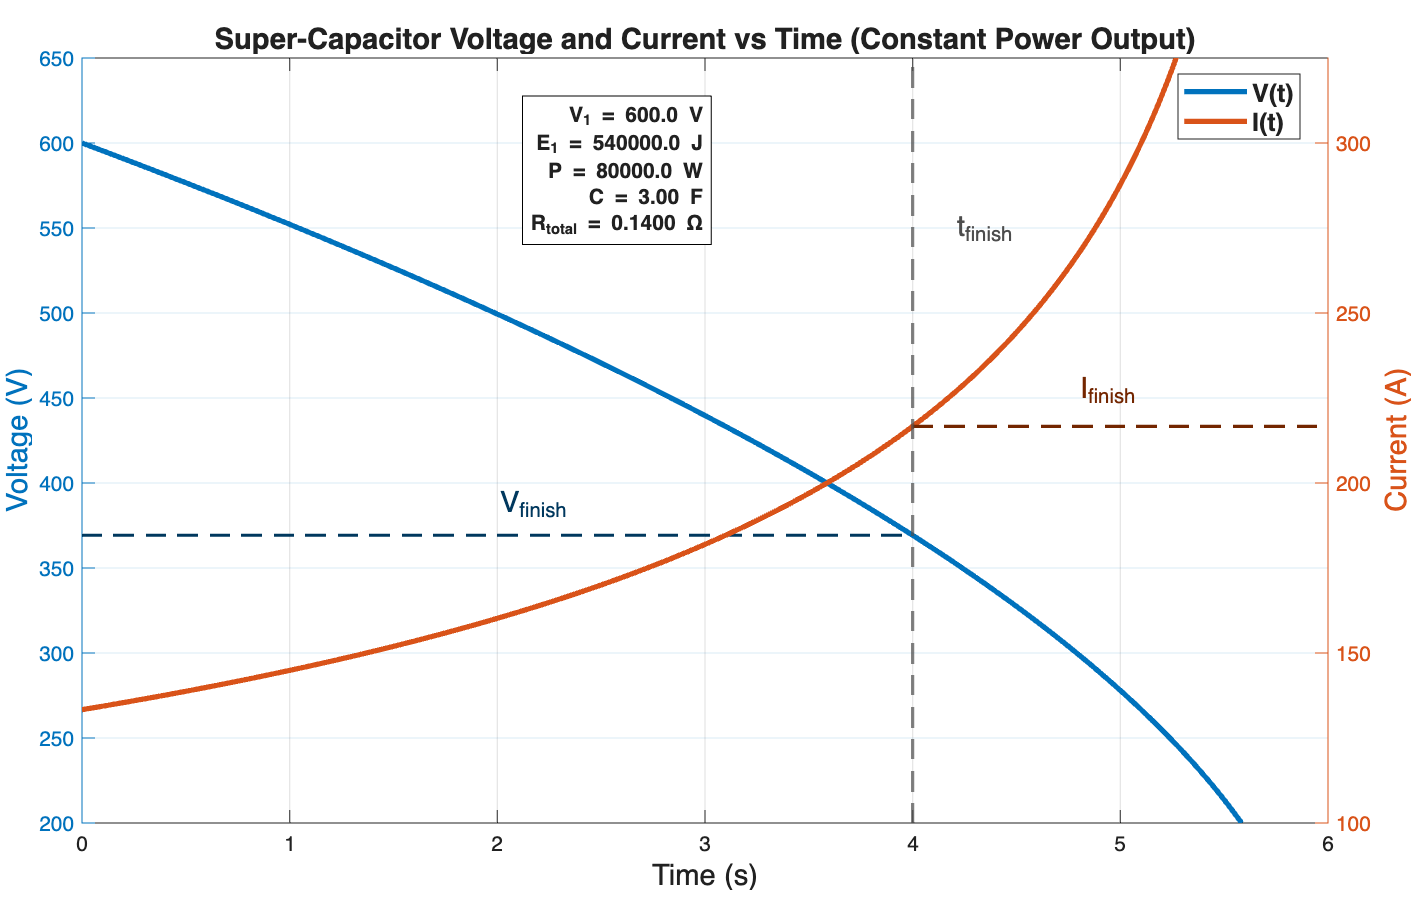
\includegraphics[width=1\textwidth]{figures/Supercapcaitor_discharge.png}
    \caption{Selected supercapacitor (SC1) discharge characteristics showing voltage and current evolution over time during constant 80 kW power discharge.}
    \label{fig:supercap_discharge}
\end{figure}

Figure \ref{fig:supercap_discharge} shows the voltage and current evolution during a constant 80 kW power discharge, giving a conservative estimate. The voltage starts at 600 V and drops to 369 V at the end of the event, set by $t_{finish}=4\,\text{s}$, confirming the expected voltage sag due to both capacitive discharge and resistive losses. The current increases to 217 A, acceptable thermally for short bursts.

\subsection{Tolerance Analysis}

The supercapacitor datasheet gives a capacitance tolerance of +0--20\% (typically +5--10\%). This tolerance dominates electrical spread and therefore defines the binning benefit analysis.

Cells are supplied in packs of 90, requiring purchase of three packs and selection of the best 200 cells. For this event, selection is simplified to maximizing capacitance rather than minimizing variance because balancing heat is not expected to be the limiting factor.

The cell capacitances are modelled using a beta distribution:
\begin{equation*}
T = 0.2*Beta(\alpha = 3, \beta = 5)
\end{equation*}

Selecting the highest cells, the expected accumulator capacitance is calculated using Equation~\eqref{eq:series_capacitance}.

Performing this Monte Carlo binning simulation to find average mean total capacitance and capacitance range, we obtain the following improvements to our initial model:

\begin{table}[htbp]
    \centering
    \caption{Accumulator performance comparison for nominal and binned (average) capacitance scenarios. Relative differences are reported against the nominal case. Constants: $P_{const}=80\,\mathrm{kW}$, $V_{total}=600\,\mathrm{V}$, $t_{finish}=4\,\mathrm{s}$, $R_{total}=0.14\,\Omega$.}
    \label{tab:capacitance_binning_results}
    \footnotesize
    \begin{tabular}{|l|c|c|c|}
        \hline
        \textbf{Metric} & \textbf{Nominal} & \textbf{Binned} & \textbf{Difference} \\
        \hline
        Capacitance (F) & 3.00 & 3.26 & +8.7\% \\
        Initial Energy (kJ) & 540 & 587 & +8.7\% \\
        Minimum Voltage (V) & 369 & 393 & +6.6\% \\
        Maximum Current (A) & 217 & 203 & -6.2\% \\
        Capacitance Range & 0\% & 10\% & \\
        \hline
    \end{tabular}
\end{table}

\subsection{Technology Selection Decision}

The two remaining candidates (EDLC and LiPo) are compared on mass, volume, cost, electrical performance, availability and complexity. High-power LiPo remains the benchmark because it is widely used in Formula Student. Comparison proceeds via quantifiable metrics of mass and volume. Cost cannot be quantified accurately due to the ambiguity in pricing for LiPo cells. Electrical performance should be similar if our criteria is met, whilst availability and complexity will be considered later as qualitative factors.

\begin{table}[htbp]
    \centering
    \caption{Comparison of EDLC supercapacitor and high-power Li-Po battery technologies \cite{batpac2022manual}. Weighted scoring system applied. LiPo wins by 4.0\% overall score, driven by volume advantages.}
    \label{tab:tech_comparison}
    \footnotesize
    \begin{tabular}{|l|c|c|l|}
        \hline
        \textbf{Technology} & \makecell{\textbf{Mass*} \\ \textbf{(kg)}} & \makecell{\textbf{Cell Volume} \\ \textbf{(L)}} & \textbf{Evaluation Method} \\
        \hline
        EDLC Cap. & 29.8 & 22.4 & Bottom-Up Estimate \\
        \arrayrulecolor{gray!30}\hline\arrayrulecolor{black}
        LiPo Battery & 33.1 & 12.5 & Top-Down Estimate \\
        \hline
        \hline
        \multicolumn{4}{|c|}{\textbf{Weighted Scoring Analysis}} \\
        \hline
        \textbf{Technology} & \textbf{Mass (3×)} & \textbf{Volume (1×)} & \textbf{Total Score} \\
        \hline
        EDLC & 3.00 & 0.56 & 3.56 \\
        \arrayrulecolor{gray!30}\hline\arrayrulecolor{black}
        LiPo & 2.70 & 1.00 & 3.70 \\
        \hline
        \textbf{Best} & \textbf{EDLC} & \textbf{LiPo} & \cellcolor{green!20}\textbf{LiPo} \\
        \hline
        \multicolumn{3}{|r|}{\textbf{LiPo Advantage:}} & \textbf{+4.0\%} \\
        \hline
    \end{tabular}
\end{table}

Two different methodologies are used to estimate mass and volume for the two technologies. For LiPo, the top-down BatPac simulation tool \cite{batpac2022manual} determines a mass-sensitive pack design. Inputs characterise both the FS regulations and the acceleration focus whilst retaining physical accuracy. An asterisk is placed next to mass in the table, as this is not total mass (which cannot yet be determined) but the sum of cell mass and other technology-specific masses. For LiPo this includes heavier pack hardware and thermal management, whilst for SC only lighter pack hardware weight is included. The supercapacitor cell mass and volume are calculated using a bottom-up approach based on the selected cell (SC1) specifications \cite{sech-c46w-3r0-0600}. Whilst LiPo pouch cells can be more tightly packed than cylindrical SC cells, they require more mechanical support, so cell volume is an accurate relative indicator of total volume for this comparison.

A weighted scoring system is applied using the following formulation:
\begin{equation*}
\text{Score} = \frac{\text{Best Value in Category}}{\text{Component Value}} \cdot \text{Weight}
\end{equation*}

A 70-30 weighting is typically applied for mass and volume, as mass has a higher impact on performance. Volume's biggest impact is the increased aerodynamic drag which it introduces. However, for this acceleration-only application, where initial speeds are low, this has a less significant effect, hence the weightings have been adjusted to 75-25 (or 3-1) to reflect this appropriately.

Whilst LiPo is advantageous in our weighted scoring analysis, it does not consider qualitative factors. The increased complexity of chemical cells introduces additional safety and thermal management challenges. In addition, availability and pricing uncertainty introduce risk to the project timeline and budget. Hence, SCs were selected, as the minor quantitative advantages of LiPo do not justify these qualitative disadvantages.

\section{Electrical System Design}

\subsection{System Architecture Overview}

Figure~\ref{fig:electronics_architecture} shows the top-level accumulator architecture. This section is structured from power-path implementation to supervisory control: busbar design, safety design, monitoring and control, and finally system integration. The architecture consists of five high-voltage (HV) segments, each monitored by AMS slaves (MC33771), communicating with the AMS master (FRDM33664BEVB) via the MC33664 TPL interface \cite{nxp-mc33771-ds}. The low-voltage (LV) control domain interfaces to the vehicle ECU (STM32 Nucleo-F4 \cite{stm32-nucleo-f4}) over CAN, using the SN65HVD230 transceiver \cite{ti-sn65hvd230-ds}. Additional key components include Bussmann 170M1759 fusing at inter-segment \cite{eaton-bussmann-170m1759-ds}, and an EarthX ETX12A 12 V supply battery \cite{earthx-etx12a-ds}. External charging and vehicle shutdown-chain implementation are outside the scope of this section.

\begin{figure}[!htbp]
    \centering
    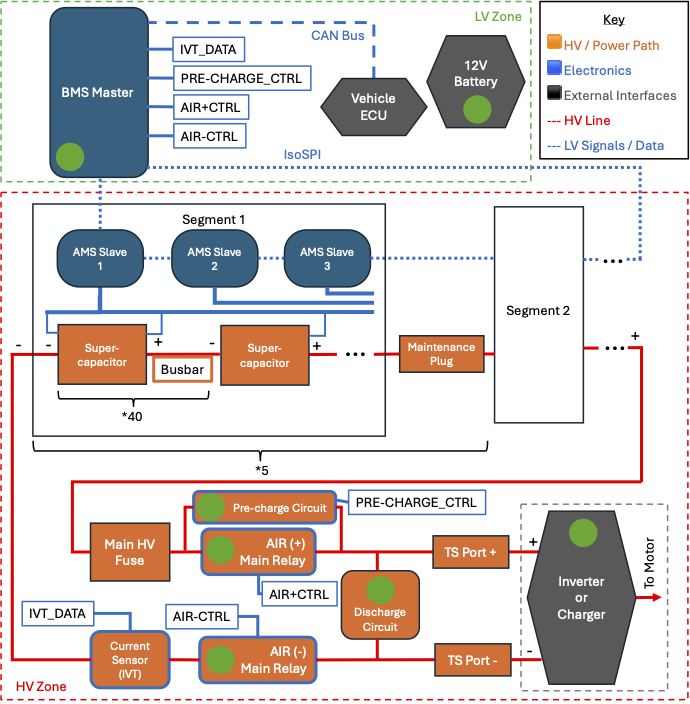
\includegraphics[width=0.9\textwidth]{figures/schematics/Electronics_architecture.png}
    \caption{Top-level electrical system architecture showing energy flow from supercapacitor cells through busbars and segments to the inverter, alongside control and communication pathways within the AMS. Green dots represent 12V battery connection}
    \label{fig:electronics_architecture}
\end{figure}

%TODO: Add the source used to define/justify this architecture diagram and interface partitioning.

\subsection{Busbar Design}

Supercapacitors are connected via busbars rather than direct cell-to-cell welding for thermal expansion management and assembly accessibility. Busbar material selection minimises $\rho_{e} \cdot \rho_{m}$, where $\rho_{e}$ is electrical resistivity and $\rho_{m}$ is mass density. Although copper exhibits superior electrical performance, aluminium 1005 was specified for compatibility with aluminium cell terminals.

Busbar connection area is matched to the terminal diameter, $d_{t}$, with average busbar length $L$ and target resistance per connection, $R$. The required thickness is calculated as:
\begin{equation*}
t = \frac{\rho_{e} L}{R d_{t}} = \frac{\left(2.8 \times 10^{-8}\,\Omega\,\text{m}\right)\left(50 \times 10^{-3}\,\text{m}\right)}{\left(0.1 \times 10^{-3}\,\Omega\right)\left(10 \times 10^{-3}\,\text{m}\right)} = 1.41\,\text{mm} \approx 1.45\,\text{mm} \text{ (standard 15 gauge)}
\end{equation*}

\subsection{Safety Design}

Grounding is treated as a floating HV system with insulation monitoring against chassis (FS-EV~4.3.1). Fuse placement is integrated per segment to localise faults and satisfy FS-EV~3.2.1 and FS-EV~3.2.7. For EMI robustness and rule-compliant layout practice, communication wiring follows segregated HV/LV routing to satisfy FS-EV~4.3.3 physical separation requirements. Any external AMS master to vehicle ECU or diagnostic connection is implemented with galvanic isolation in accordance with FS-EV~4.3.2. Vehicle-level shutdown-chain implementation, AIR actuation hardware, and charging safety circuitry are outside the scope.

\subsection{Monitoring and Control Systems}
\label{subsec:electrical_design}

\begin{figure}[!htbp]
    \centering
    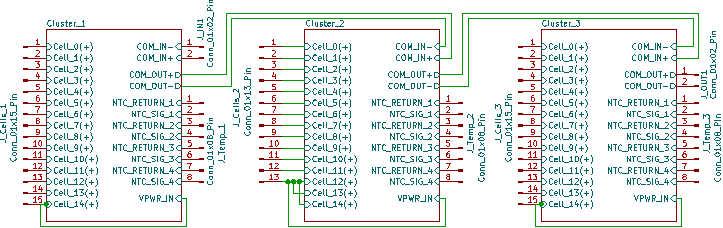
\includegraphics[width=\textwidth]{figures/schematics/PCB.pdf}
    \caption{Complete segment AMS PCB schematic showing MC33771 topology for 40-cell segment monitoring.}
    \label{fig:pcb_schematic}
\end{figure}

The controller IC is powered directly by the cells themselves via the \texttt{VPWR} pins and therefore floats at the segment potential. The daisy-chain interface follows TPL pin mapping, with \texttt{COM\_IN} receiving data from the lower segment and \texttt{COM\_OUT} forwarding data to the upper segment.

\begin{figure}[!htbp]
    \centering
    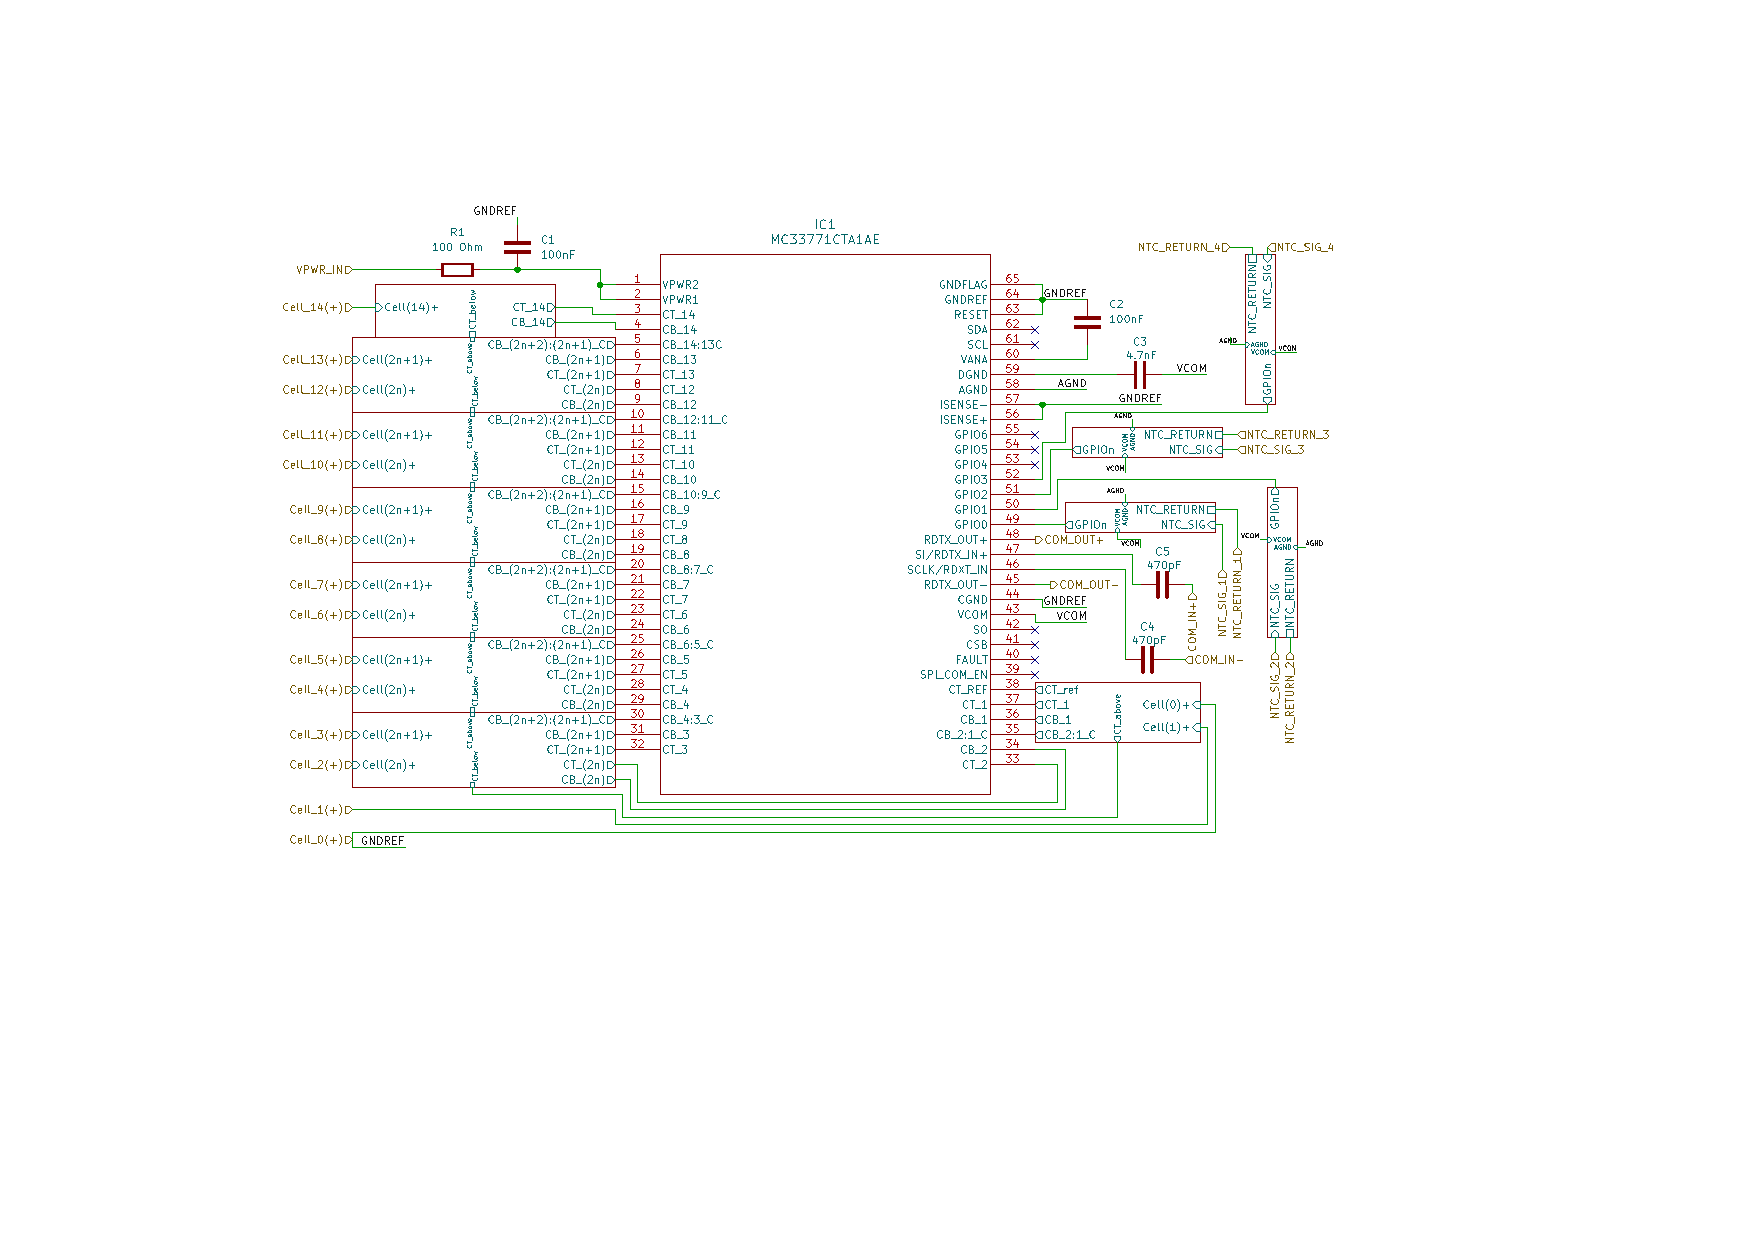
\includegraphics[width=\textwidth]{figures/schematics/PMIC2.pdf}
    \caption{Singular Cluster (1) schematic showing voltage and temperature monitoring with isolation and protection features.}
    \label{fig:pmic}
\end{figure}

\textbf{AMS architecture and communication:} The monitoring network adopts a scalable master-slave topology using NXP MC33771 controllers across five accumulator segments \cite{nxp-mc33771-ds}. Communication is implemented with the NXP Twisted Pair Link (TPL) interface via the MC33664, whose current-mode transmission provides strong immunity to inverter-generated EMI \cite{nxp-mc33664-ds}. Galvanic domain separation in the daisy chain is maintained using high-voltage safety capacitors ($C4$, $C5$), which couple communication across stacked segment voltage domains while blocking DC transfer.

The TPL bus is implemented as a single-ended daisy chain from the AMS master to the first AMS slave. The architecture uses three AMS slaves per segment across five segments (15 slaves total), with data forwarded stage-by-stage via \texttt{COM\_OUT} to \texttt{COM\_IN}. The end of the chain is terminated using the NXP-recommended end-of-line network, including a termination resistor, to ensure signal integrity and avoid reflections.

Each slave device performs segment voltage and temperature acquisition and reports diagnostic status to the AMS master. The AMS master (FRDM33664BEVB) executes pack-level limit checks, aggregates faults, and communicates accumulator status to the vehicle ECU (STM32 Nucleo-F4).

\textbf{Voltage sensing and balancing:} Cell voltage sensing uses an anti-aliasing filter with $R = 100\,\Omega$ (R6, R7 in Figure~\ref{fig:signal_conditioning}a) and $C = 47\,\text{nF}$ (C8, C9 in Figure~\ref{fig:signal_conditioning}a). The corresponding cutoff frequency
\begin{equation*}
f_c = \frac{1}{2\pi R C} = \frac{1}{2\pi (100)(47 \times 10^{-9})} \approx 33.8\,\text{kHz},
\end{equation*}
which attenuates high-frequency inverter switching content while preserving measurement bandwidth for pack diagnostics. Based on the binned-cell capacitance spread of up to 10\% (Table~\ref{tab:capacitance_binning_results}), passive balancing is required to control inter-cell voltage divergence. Passive balancing is implemented through switchable resistors with $R_{bal} = 33\,\Omega$ (R5, R8, R9 in Figure~\ref{fig:signal_conditioning}a). At a nominal maximum cell voltage of 3 V, the corresponding balancing current is $I_{bal} \approx 91\,\text{mA}$, and the dissipation per balancing branch is
\begin{equation*}
P_{diss} = \frac{V_{cell}^{2}}{R_{bal}} = \frac{(3\,\text{V})^{2}}{33\,\Omega} \approx 0.27\,\text{W}.
\end{equation*}

This thermal load requires resistor packages with sufficient margin, so the format 1210, rated at 0.5\,W, was chosen for stable operation during balancing intervals.

\begin{figure}[!htbp]
    \centering
    \begin{subfigure}[b]{0.65\textwidth}
        \centering
        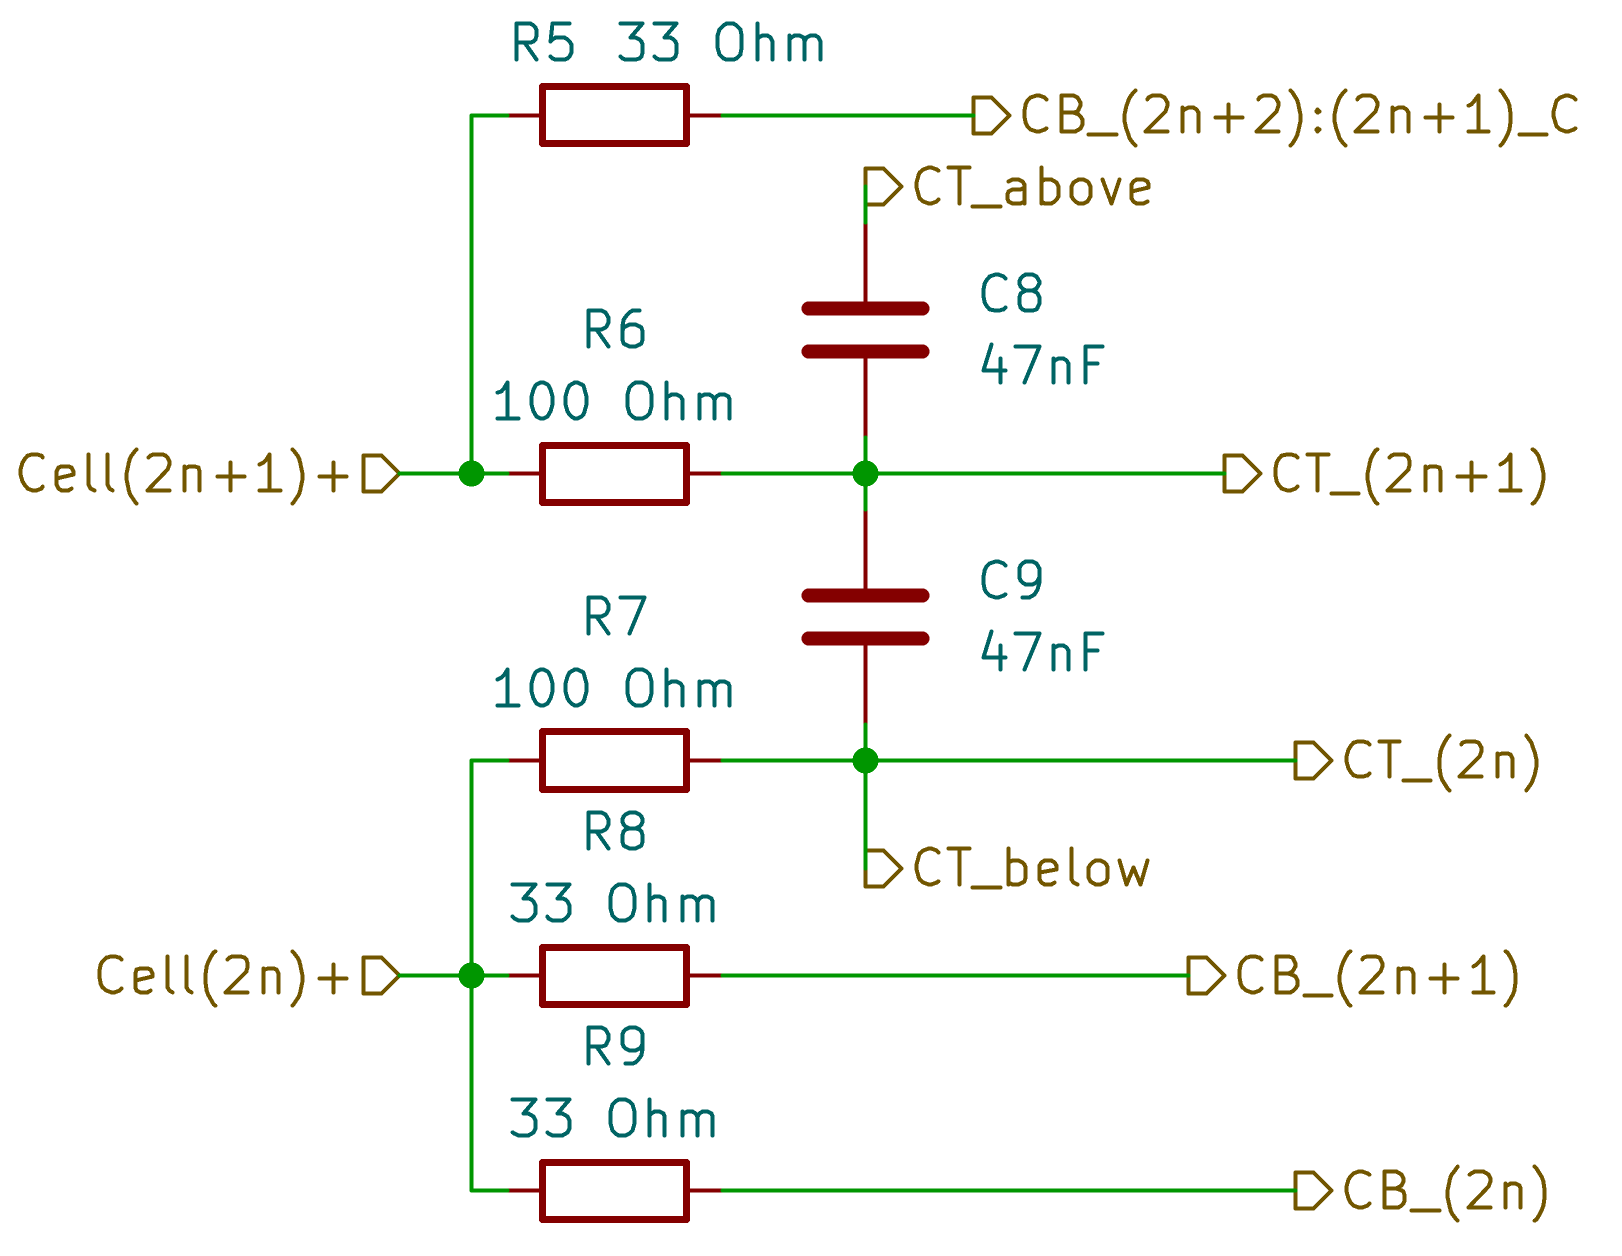
\includegraphics[width=\textwidth]{figures/schematics/VoltageFilter.png}
        \caption{Voltage sensing and filtering circuit.}
        \label{fig:voltage_filter}
    \end{subfigure}
    \hfill
    \begin{subfigure}[b]{0.28\textwidth}
        \centering
        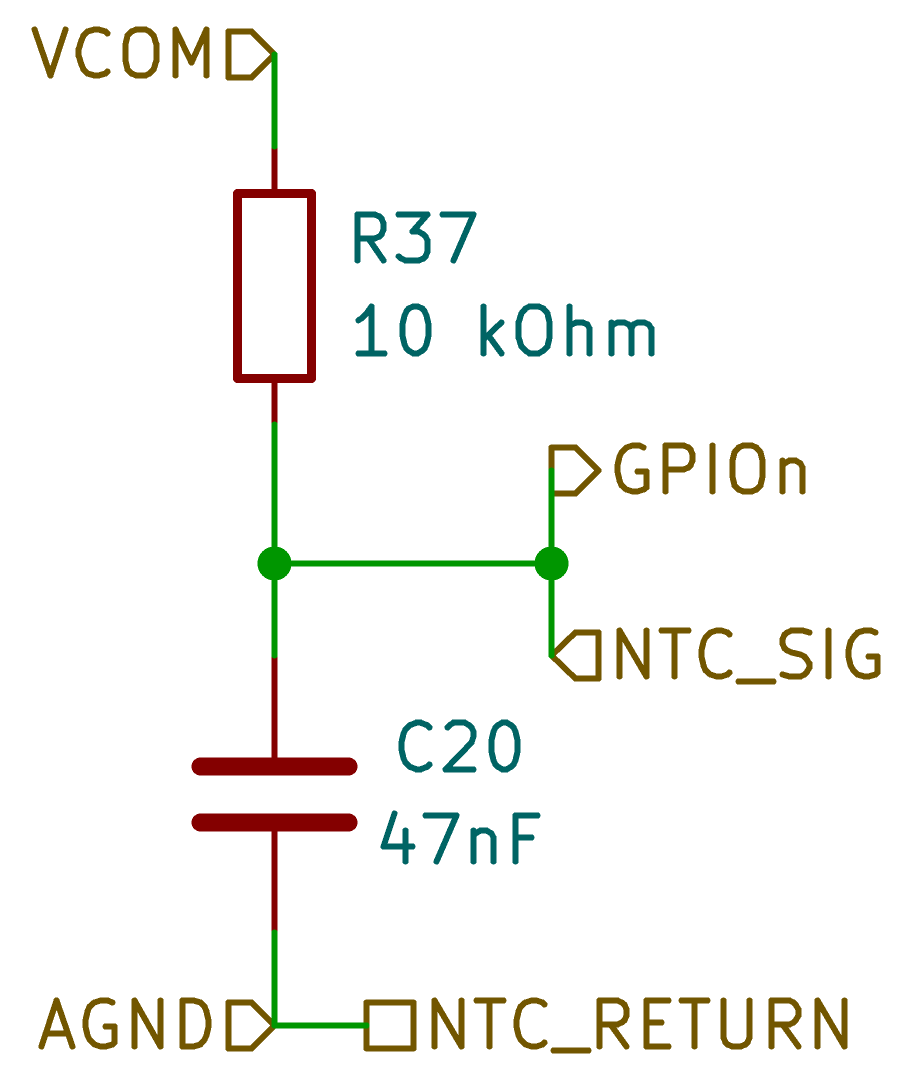
\includegraphics[width=\textwidth]{figures/schematics/TemperatureSensor.png}
        \caption{Temperature sensing circuit.}
        \label{fig:temperature_sensing}
    \end{subfigure}
    \caption{Signal conditioning circuits for AMS monitoring}
    \label{fig:signal_conditioning}
\end{figure}

%TODO: Rerender graphics so that label text is much larger

\textbf{Temperature monitoring and protection:} Temperature channels are conditioned with an RC input filter ($R=10\,\text{k}\Omega$, $C=47\,\text{nF}$), implemented as R37 \& C20 in Figure~\ref{fig:signal_conditioning}b. This suppresses transient noise that could otherwise cause false over-temperature flags. NTC thermistors are connected directly to \texttt{GPIO} measurement channels, and cell temperature is reconstructed from this voltage. Sensors are placed on 30\% of the cells to satisfy temperature monitoring requirements (FS-EV~5.8.4). The protection strategy applies a hard fault response using the AIR when any monitored cell temperature exceeds $T > 60^\circ\text{C}$ (FS-EV~5.8.5), with AMS-triggered shutdown behavior as required by FS-EV~5.8.7.

\subsection{System Integration}

System integration defines how the accumulator monitoring subsystem interfaces with the rest of the vehicle once local sensing and protection functions are implemented. In this design, the integration point is the AMS master-to-ECU CAN interface, through which pack-level status and fault state should be communicated for vehicle-level decision making.

The AMS master and ECU must operate in the LV domain and should be supplied from the vehicle 12 V system, while all segment electronics should remain referenced to their local HV potentials. Galvanic isolation must be maintained at external interfaces (FS-EV~4.3.2), and TS/LV physical segregation preserved in routing and packaging (FS-EV~4.3.3). Within this report scope, the integration boundary ends at the AMS master to ECU status interface; hence, vehicle shutdown-chain actuation logic, charger-side functions, and full firmware message implementation are not included.

\section{Mechanical Design and Packaging}
The electrical requirement of 200 series-connected cells necessitates segmentation into 5 modules of 40 cells each to maintain voltage domains within FS-EV regulations. All segments are housed within a single Accumulator Container (AC), separated by internal insulating walls.

\subsection{Segment Design}

%TODO: Rerender so it is naturally landscape and fits better on the page.
\begin{figure}[!htbp]
    \centering
    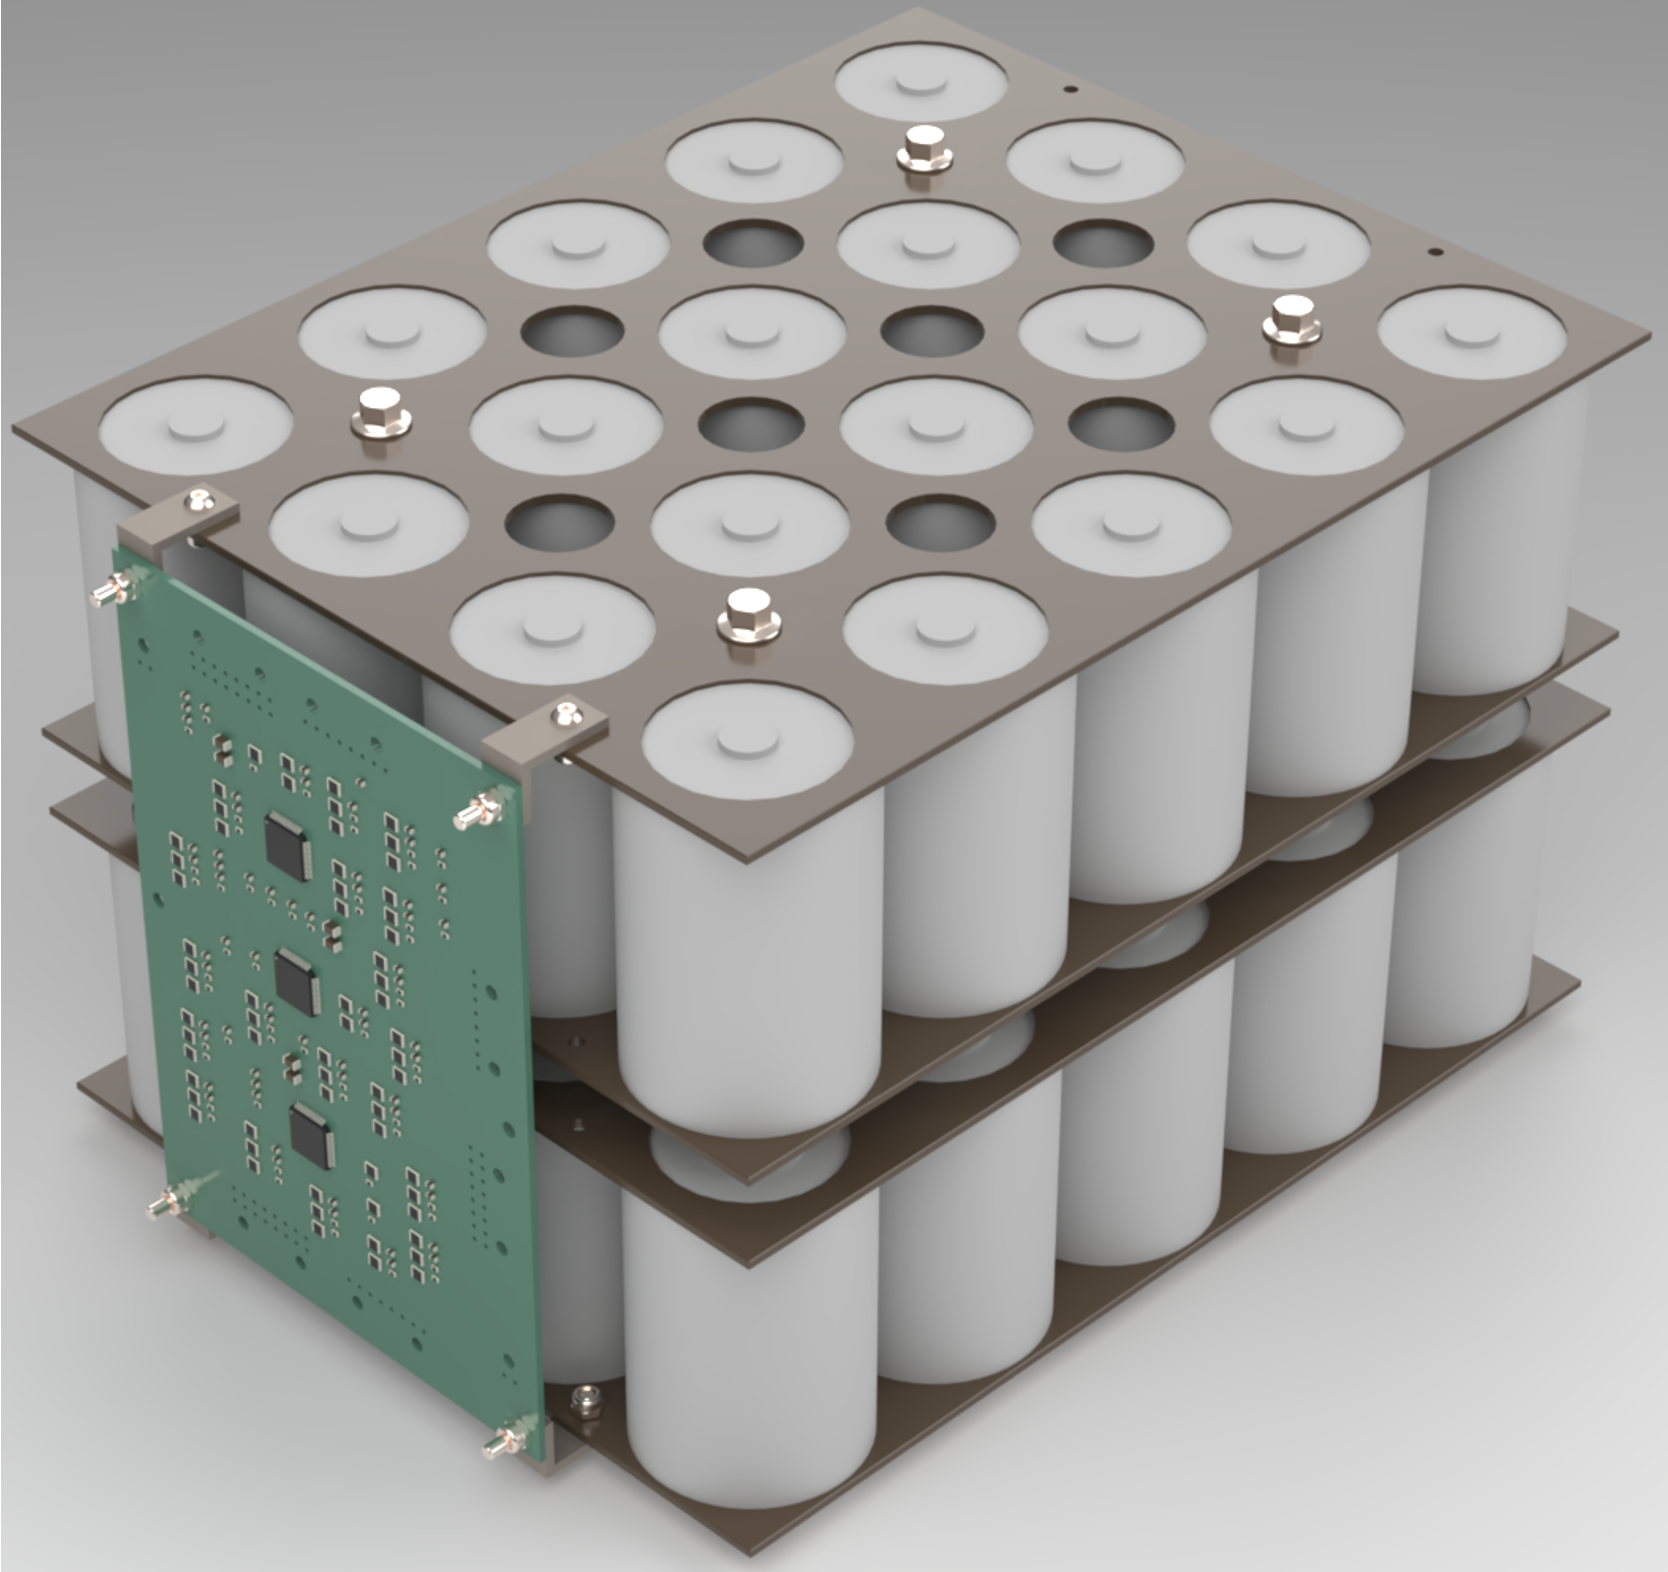
\includegraphics[width=0.8\textwidth]{figures/renders/segment.png}
    \caption{Accumulator segment design without enclosure and busbar connections.}
    \label{fig:main_segment}
\end{figure}

Segment design prioritises modularity and replicability, with each segment containing series-connected cells secured by mechanical holders and electrically isolated by spacing. Each segment comprises two 20-cell sub-modules in a 5×4 rectangular grid, leaving a central corridor for sensing and wiring.

Although honeycomb packing is generally denser, it provides only about 1\% volume reduction once constrained to cuboid envelope, so the rectangular layout is retained for simplicity.

The PCB layout (detailed in Section~\ref{subsec:electrical_design}) is positioned to fit within the segment depth and centered to facilitate harness routing and cell connection while enabling mechanical accessibility via bracket-based mounting to the FR4 matrix board. PCB peripheral spacing accommodates cable routing.

Fuses are mounted to the casing and their exact position varies by segment because of inter-segment packaging constraints. Busbar topology is consistent, but routing varies to support fuse placement.

\subsection{Accumulator Container (AC) \& Integration with Vehicle}

\begin{figure}[!htbp]
    \centering
    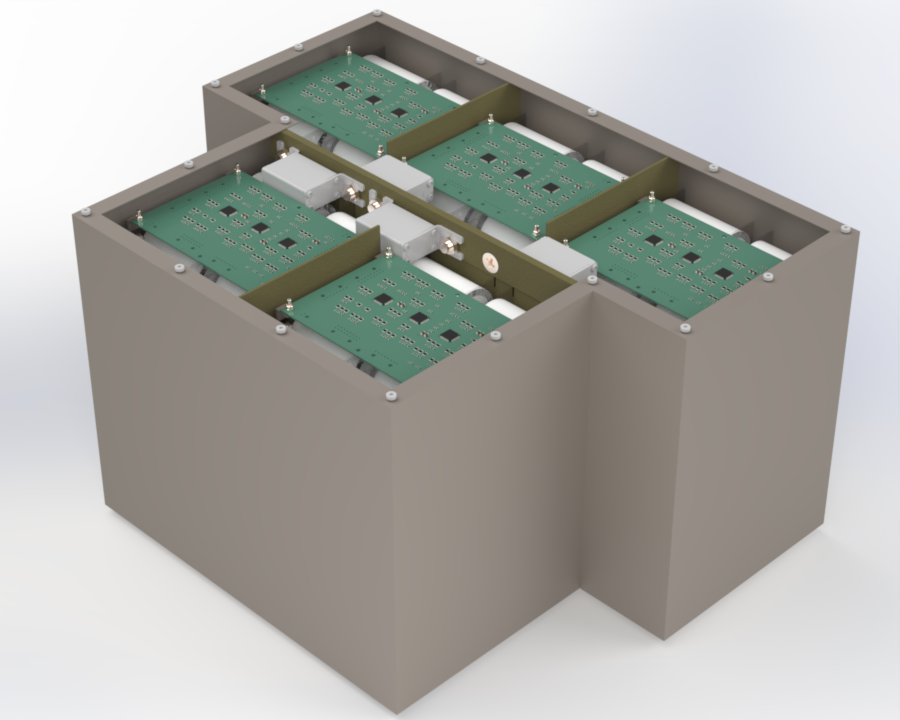
\includegraphics[width=0.9\textwidth]{figures/renders/main4.png}
    \caption{Accumulator design with lid removed for visibility.}
    \label{fig:main_accumulator}
\end{figure}

% TODO: Change Rendering so that the actual floor is at the bottom of the image, then adjust paragraph accordingly
% Consider placing next to the other segment rendering to save space

The accumulator is placed between driver and motor, below the inverter, to reduce HV cable mass and move mass near the rear axle. This packaging envelope drives the 3--2 segment arrangement.

%TODO: Add reference to Toby's section showing the accumulator placement within the vehicle.

The external casing is fabricated from stainless steel featuring 0.9 mm walls and a 1.2 mm floor to meet FS-EV~4.4.2 regulations. The three-piece assembly (removable bolted lid, welded lower shell, and base floor) enables service access while maintaining structural integrity.

Detailed manufacturing process planning, quality control workflow, and full BOM costing are not expanded in this report and are deferred to implementation documentation.

\section{Results and Discussion}



\subsection{Comparison with LiPo Baseline}

\begin{table}[htbp]
    \centering
    \caption{Comparison of EDLC supercapacitor, using results from design analysis, and high-power Li-Po battery technologies, using motorsport adapted simulation results \cite{batpac2022manual}. Weighted scoring system applied. Tie between the two technologies.}
    \label{tab:results_comparison}
    \footnotesize
    \begin{tabular}{|c|l|l|l|}
        \hline
        \textbf{Technology} & \makecell{\textbf{Mass} \\ \textbf{(kg)}} & \makecell{\textbf{Volume} \\ \textbf{(L)}} & \textbf{Evaluation Method} \\
        \hline
        EDLC Cap. & 36.0 & 44.5 & Design \\
        \arrayrulecolor{gray!30}\hline\arrayrulecolor{black}
        LiPo Battery & 40.3 & 30.3 & BatPac Sim \\
        \hline
        \hline
        \multicolumn{4}{|c|}{\textbf{Weighted Scoring Analysis}} \\
        \hline
        \textbf{Technology} & \textbf{Mass (3×)} & \textbf{Volume (1×)} & \textbf{Total Score} \\
        \hline
        EDLC & 3.00 & 0.68 & 3.68 \\
        \arrayrulecolor{gray!30}\hline\arrayrulecolor{black}
        LiPo & 2.68 & 1.00 & 3.68 \\
        \hline
        \textbf{Best} & \textbf{EDLC} & \textbf{LiPo} & \cellcolor{orange!20}\textbf{Tie} \\
        \hline
    \end{tabular}
\end{table}

The results table~\ref{tab:results_comparison} now evaluates the final design against the LiPo baseline, moving to a more accurate model than the initial technology comparison~\ref{tab:tech_comparison}. Mass and volume results for the SC solution are taken directly from the CAD model design. LiPo baseline results have been adjusted to reflect a complete pack design, again with the appropriate motorsport mass adjustments. The volume cannot be as easily adjusted, so the given cell volume is scaled by the CtP ratio of pouch cells in FS designs (0.413) \cite{epp_multiphysical_battery}. The LiPo and SC solutions now tie on the weighted score, so cost becomes the deciding factor once the final BOM costings are added and compared with typical LiPo pricing from FS teams.
%TODO add sources for this and then a rough cost multiplicative factor.
The same qualitative factors discussed previously still apply. Given lower supply risk, pricing ambiguity, and system complexity, it can be strongly argued that the SC solution is superior to the LiPo baseline for this project context.

\subsection{Design Criteria Achievement}
\label{sec:design_criteria_achievement}
The finalised design is verified against the requirement IDs in Table~\ref{tab:design_requirement_ids}, using the LiPo comparison in Table~\ref{tab:results_comparison} as the supporting evidence for the minimisation targets:

\begin{table}[htbp]
    \centering
    \caption{Requirement verification matrix for final design outcomes.}
    \label{tab:design_verification_matrix}
    \footnotesize
    \setlength{\tabcolsep}{4pt}
    \renewcommand{\arraystretch}{0.95}
    \begin{tabular}{|c|p{5cm}|p{7.5cm}|p{2cm}|}
        \hline
        \textbf{ID} & \textbf{Target} & \textbf{Evidence} & \textbf{Status} \\
        \hline
        R1 & $80\,\text{kW}$ & 80 kW sustained across the event & Met \\
        R2 & $320\,\text{kJ}$ & 320 kJ available with manageable current & Met \\
        R3 & Minimise mass, volume, cost, and procurement risk & Table~\ref{tab:results_comparison} gives a tie on total score; qualitative factors favour SC solution & Partially evidenced \\
        \hline
    \end{tabular}
\end{table}

%TODO: somehow justify the cost point
%TODO: reference operating window from results of Harry Sims. 
%TODO: add a short assumptions/limitations paragraph (event profile, voltage window, thermal simplifications).

\section{Future Improvements and Conclusion}

\subsection{Refinements for Implementation}
The design establishes a coherent architecture suitable for prototyping and integration. Key refinement priorities for implementation include: (1) detailed thermal analysis; (2) AMS firmware development; (3) manufacturing partner engagement for cost and lead-time validation; and (4) comprehensive electrical \& mechanical testing.

\subsection{Future Improvements}

Our current implementation, during the race, the car is only ever traction or power limited. For the accumulator design, the major optimisation opportunity to improve performance is to reduce mass. The following approaches could be considered to achieve this:
%TODO: insert conclusion from Harry's sims.
\begin{itemize}
    \item A lighter SC cell (SC2), albeit with increased voltage sag, due to lower capacity or higher ESR. This would require more accurate thermal management due to increased power losses.
    \item A hybrid/asymmetric SC cell, which would strike a balance between SC's and LiPo's energy and power densities. However, to reduce the risk from the limited commercial availability, a more active procurement strategy would be required, including early engagement with suppliers to secure cells and detailed testing to validate performance claims.
\end{itemize}

\subsection{Conclusion}
The accumulator system design successfully combines proven supercapacitor technology with modular electrical and mechanical architecture to meet Formula Student requirements, optimised for the acceleration application. The analysis demonstrates that SCs provide equally effective quantitative performance as LiPo batteries, whilst providing a more affordable and reliable solution. The design provides a well-thought-out system that could be manufactured and integrated into the vehicle. Subsequent development phases should focus on prototype validation, thermal characterisation in realistic vehicle operating conditions, and iterative refinement based on test data.

\compactbib
